\chapter{Personalized PageRank for Graph Embedding}
\section{Introduction}
\subsection{Our contributions}
\subsection{Organization of the chapter}
\section{PageRank}
The PageRank score was briefly introduced in section \ref{subsec:Intro_centrality}. We propose here an in-depth study of this metric and its personalized version, its theoretical properties and its practical computation.

Let's first recall the definition of the PageRank score.

\subsection{Equivalent definitions of PageRank and PPR} \label{subsec:ppr_definitions}
\subsubsection{PageRank}
The first definition of PageRank with a parameter $\alpha \in [0, 1)$ was that of a random walk with restart in the graph. The walker starts from a vertex drawn uniformly at random and at each step, it makes one of the following two moves:
\begin{description}
    \item[Restart] The walker chooses any vertex of the graph at random and jumps to it.
    \item[Walk] The walker draws uniformly at random one of the neighbors (out-neighbors in the case of directed graphs) of the vertex it is on and goes to that neighbor.
\end{description}

At each step, the probability to restart is $\alpha$ and the probability to walk is $1-\alpha$. Let's note $p_i \in \realset^n$ the vector that, for each vertex, contains the probability of being on that vertex at step $i$. The random walk is defined by the following sequence:
\begin{equation}\label{eq:pr_def_as_sequence}
    \begin{cases}
        p_0 = \frac{1}{n}\ones\\
        p_{i+1}^\top = \alpha \underbrace{p_0^\top}_{\text{Restart}} + (1-\alpha)\underbrace{p_i^\top M}_{\text{Walk}}
    \end{cases}
\end{equation}
where $\ones \in \realset^n$ is the vector of which all elements are $1$.

\begin{property}\label{prop:pr_def_as_equation}
    The sequence defined at equation \ref{eq:pr_def_as_sequence} converges to the vertex $\pi$ defined by 
    \begin{equation}\label{eq:pr_def_as_equation}
        \pi^\top = \alpha p_0^\top + (1-\alpha)\pi^\top M
    \end{equation}
\end{property}
\begin{proof}
    Let $f : \realset^n \rightarrow \realset^n$ be the iteration function, $f(x)^\top =\alpha p_0^\top + (1-\alpha)p_i^\top M$. We have 
    \begin{equation*}
        \forall x, y \in \realset^n : f(x)^\top - f(y)^\top = (1-\alpha)(x-y)^\top M
    \end{equation*}
    Since $M$ is a stochastic matrix, we have $\forall z \in \realset^n : ||z^\top M||_1 \leq ||z||_1$. Therefore we have 
    \begin{equation*}
        \forall x, y \in \realset^n : ||f(x)^\top - f(y)^\top||_1 \leq (1-\alpha)||(x-y)||_1
    \end{equation*}
    This proves that $f$ is a contraction mapping on $\realset^n$ and so the Banach fixed-point theorem concludes the proof.
\end{proof}

The PageRank vector of the graph $G$ is the asymptotic limit of the sequence defined in equation \ref{eq:pr_def_as_sequence}, i.e. it is the vector $\pi$ defined in equation \ref{eq:pr_def_as_equation}.

\begin{property}\label{prop:pr_def_as_series}
    The PageRank vector $\pi$ defined in equation \ref{eq:pr_def_as_equation} can be equivalently written as the series
    \begin{equation}\label{eq:pr_def_as_series}
        \pi^\top = \alpha \sum_{i = 0}^{+\infty} (1-\alpha)^i p_0^\top M^i
    \end{equation}
\end{property}
\begin{proof}
    We can show by induction that the general term of the sequence described in equation \ref{eq:pr_def_as_sequence} is
    \begin{equation*}
        p_i = (1-\alpha)^i p_0^\top M^i + \alpha \sum_{j = 0}^{i-1} (1-\alpha)^j p_0^\top M^j
    \end{equation*}

    It has already been shown that the sequence converges. 
    
    Given that $\lim_{i \to +\infty} ||(1-\alpha)^i p_0^\top M^i||_1 = 0$ then
    \begin{equation*}
        p_i \sim_{i \to +\infty} \alpha \sum_{i = 0}^{i-1} (1-\alpha)^i p_0^\top M^i
    \end{equation*}
\end{proof}

\subsubsection{Personalized PageRank}
In a graph $G = \{V, E\}$, the Personalized PageRank (PPR) vector $\pi_u$ of a vertex $u \in V$ with parameter $\alpha$ is the asymptotic vector of the sequence defined by 
\begin{equation}\label{eq:ppr_def_as_sequence}
    \begin{cases}
        p_0 = e_u\\
        p_{i+1}^\top = \alpha p_0^\top + (1-\alpha)p_i^\top M
    \end{cases}
\end{equation}
with $e_u \in \realset^n$ the vector of which the only non-zero element is a $1$ at the $u$\textsuperscript{th} position.

This definition is identical to equation \ref{eq:pr_def_as_sequence} except for the first term. It is easy to see that properties \ref{prop:pr_def_as_equation} and \ref{prop:pr_def_as_series} also apply.

\begin{definition}[Personalized PageRank (PPR) matrix]
    The \define{Personalized PageRank matrix} $\Pi \in \realset^{n \times n}$ of a graph $G = \{V, E\}$ with parameter $\alpha$ is the matrix of which each line is the PPR vector of the related vector of the graph.
\end{definition}

We know from properties \ref{prop:pr_def_as_equation} and \ref{prop:pr_def_as_series} that
\begin{equation*}
    \pi_u^\top = \alpha e_u^\top + (1-\alpha) p_u^\top M
\end{equation*}
and
\begin{equation*}
    \pi_u^\top = \alpha \sum_{i=0}^{+\infty} (1-\alpha)^i e_u^\top M^i
\end{equation*}

We can deduce that
\begin{equation}\label{eq:ppr_mat_as_equation}
    \Pi = \alpha I + (1-\alpha)\Pi M
\end{equation}
and
\begin{equation}\label{eq:ppr_mat_as_series}
    \Pi = \alpha \sum_{i=0}^{+\infty} (1-\alpha)^i M^i
\end{equation}
where $I\in \realset^{n\times n}$ is the identity matrix.

Finally we see from equation \ref{eq:ppr_mat_as_equation} that 
\begin{equation} \label{eq:ppr_mat_as_inverse}
    \Pi = \alpha (I - (1-\alpha)M)^{-1}
\end{equation}

Note that $I - (1-\alpha)M$ is a strictly diagonally dominant matrix and hence is invertible.

\subsubsection{Interpretations}
A first interpretation of the PageRank and Personalized PageRank vectors has been given in its definition. We propose two other interpretations.

In the first new interpretation, a content (e.g. information, liquid...) flows from the vertices in $p_0$. At each step, a fraction $\alpha$ of the still-flowing content it kept or dissipated on its current vertex and the rest divides equally to keep flowing to the neighbors. The PageRank or PPR vector is the proportion of the content that have been kept or dissipated on each the vertex, i.e. the exposure of each vertex to the content.

The second interpretation comes directly from equation \ref{eq:ppr_mat_as_series} and uses another random walk. In this new random walk, the initial position of the walker is selected as in the definition of PageRank or PPR but then the actions of the walker are one of these two:
\begin{description}
    \item[Stop] The walker stops walking and the random walk ends
    \item[Walk] The walker draws uniformly at random one of the neighbors (out-neighbors in the case of directed graphs) of the vertex it is on and goes to that neighbor.
\end{description}

The probability of stopping is $\alpha$. The value for a vertex $v$ in the PageRank or PPR vector is the probability that the walker is on that vertex when he stops walking. This interpretation helps to understand why it is usually enough to compute only a few steps of the walk to approximate the PageRank or PPR vectors. For example if $\alpha = 0.1$ then after only $66$ steps the probability that the walker is still walking is less than $10^{-3}$.

\subsection{Properties of the PPR matrix}
\begin{theorem} The multiplication of $\Pi$ with $M$ is symmetrical
    \[\Pi M = M \Pi\]
\end{theorem}
\begin{proof}
    \begin{equation*}
    \begin{split}
        \Pi M - M \Pi & = \cancel{\alpha M} + (1-\alpha)\Pi M^2 \cancel{- \alpha M} - (1-\alpha) M \Pi M\\
        & = (1-\alpha)(\Pi M - M \Pi) M
    \end{split}
\end{equation*}
so $$(\Pi M - M \Pi)(I - (1-\alpha)M) = 0_{\mathbb{R}^{n \times n}}$$ with $0_{\mathbb{R}^{n \times n}} \in \mathbb{R}^{n \times n}$ the zero matrix.

Since $(I - (1-\alpha)M)$ is invertible we deduce that
\[(\Pi M - M \Pi) = 0_{\mathbb{R}^{n \times n}}\]
\end{proof}

\begin{theorem}
    If the graph $G$ is undirected, then the matrices $D\Pi$ and $\Pi D^{-1}$ are symmetrical\todo{Mention now or later that it would allow eigendecomposition, but not studied yet}
\end{theorem}
\begin{proof}
     We first prove that $\Pi D^{-1}$ is symmetrical. We note that since $G$ is undirected, $A$ is symmetrical. We also recall that $\forall A, B$ invertible matrices, $(AB)^{-1} = B^{-1} A^{-1}$.
     
     We use the definition of $\Pi$ given by the equation \ref{eq:ppr_mat_as_inverse}. Then we have 
    \begin{equation*}
        \begin{split}
            \Pi D^{-1} &= \alpha (I - (1-\alpha) M)^{-1} D^{-1}\\
            &= \alpha (D - (1-\alpha) D \underbrace{M}_{= D^{-1} A})^{-1}\\
            &= \alpha (D - (1-\alpha) D \underbrace{A D^{-1} D}_{=M^\top D})^{-1}\\ 
            &= \alpha D^{-1}(I - (1-\alpha) M^\top)^{-1}\\
            &= D^{-1}\Pi^\top
        \end{split}
    \end{equation*}
    The proof that $D\Pi$ is symmetric follows directly from $\Pi D^{-1} = D^{-1} \Pi^\top$
\end{proof}

\begin{theorem}\label{th:dpi_pidm_symdefpos}
    If the graph $G$ is undirected, then the matrices $D\Pi$ and $\Pi D^{-1}$ are positive-definite
\end{theorem}
We note that if a matrix $\Gamma$ is symmetric and positive-definite, then there is an eigendecomposition $\Gamma = U D U^\top$ so that $U$ is a unitary matrix and $D$ is diagonal and strictly positive. Therefore the inverse matrix $\Gamma^{-1} = U D^{-1} U^\top$ is also symmetric and positive-definite. We also know from equation \ref{eq:ppr_mat_as_inverse} that the inverse of $D\Pi$ and $\Pi D^{-1}$ are respectively $\frac{1}{\alpha} \big(D^{-1} - (1-\alpha)D^{-1} A D^{-1}\big)$ and $\frac{1}{\alpha} \big(D - (1-\alpha)A\big)$. The proof will therefore consist in proving that the matrices $\big(D^{-1} - (1-\alpha)D^{-1} A D^{-1}\big)$ and $\big(D - (1-\alpha)A\big)$ are positive-definite, i.e. that the quadratic forms defined by these matrices over $\realset^n$ is an inner product.

\begin{proof}[Proof that $\big(D^{-1} - (1-\alpha)D^{-1} A D^{-1}\big)$ is positive-definite]

    $\forall x \in \realset^n$, we have
    \begin{equation*}
        \begin{split}
            x^\top \big(D^{-1} - (1-\alpha)D^{-1} A D^{-1}\big) x &= \sum_{u=1}^n \frac{x_u^2}{d_u} - (1-\alpha)\sum_{u=1}^n \sum_{v=1}^n \frac{x_u x_v}{d_u d_v} a_{uv}\\
            & = \alpha \sum_{u=1}^n \frac{x_u^2}{d_u} + (1-\alpha)\sum_{u=1}^n\big(\frac{x_u^2}{d_u} - \sum_{v=1}^n \frac{x_u x_v}{d_u d_v} a_{uv}\big)\\
            & = \alpha \sum_{u=1}^n \frac{x_u^2}{d_u} + (1-\alpha)\sum_{u=1}^n\sum_{v=1}^n\frac{x_u}{d_u}\big(\frac{x_u}{d_u} - \frac{x_v}{d_v}\big)a_{uv}\\
            & = \alpha \sum_{u=1}^n \frac{x_u^2}{d_u} + \frac{1-\alpha}{2}\sum_{u=1}^n\sum_{v=1}^n\big(\frac{x_u}{d_u} - \frac{x_v}{d_v}\big)^2a_{uv}\\
        \end{split}
    \end{equation*}
    We see that $x^\top \big(D^{-1} - (1-\alpha)D^{-1} A D^{-1}\big) x \geq 0$ and that $0$ is reached only when $x=\zeros{\realset^n}$
\end{proof}

\begin{proof}[Proof that $\big(D - (1-\alpha) A\big)$ is positive-definite]

With a similar reasoning as for $\allowbreak\big(D^{-1} - (1-\alpha)D^{-1} A D^{-1}\big)$, we get that $\forall x \in \realset^n$, we have
\begin{equation*}
    x^\top\big(D - (1-\alpha) A\big)x = \alpha \sum_{u=1}^n d_u x_u^2 + \frac{1-\alpha}{2}\sum_{u=1}^n\sum_{v=1}^n(x_u - x_v)^2a_{uv}\\ 
\end{equation*}
\end{proof}

\subsection{Computing the PPR matrix and vectors}
We note $\pi(p_0)$ the PPR vector generated from the PageRank random walk with restart using $p_0$ as the initial vector. This can be the PageRank vector, and rooted PPR vector or any PPR vector starting from a set of nodes.

The main idea of this algorithm is to build sequences $(q_i)_{i\in \naturalset}$ and $(r_i)_{i\in \naturalset}$ that maintain the following invariant
\begin{equation}\label{eq:ppr_alg_invariant}
    \forall i \in \naturalset, \big(\pi(p_0)\big)^\top = q_i^\top + r_i^\top\Pi
\end{equation}

The pseudo-code is shown as Algorithm \ref{alg:ppr_invariant}. In this algorithm, the vectors $p_i$ are the successive approximations of the PPR vector while the vectors $r_i$ are the residual values that are still to be considered in the approximation. This algorithm can be seen as a simulation of the interpretation as content flowing given in section \ref{subsec:ppr_definitions}. With that interpretation, $p_i$ is the content that has already stopped while $r_i$ represents the content that keeps flowing.

The convergence of this algorithm is guaranteed by the fact that $M$ is a stochastic matrix and hence $\forall i \in \naturalset : ||r_iM||_1 \leq ||r_i||_1$. Therefore $\forall i \in \naturalset : ||r_{i+1}||_1 \leq (1-\alpha)||r_i||_1$. $||r_i||_1$ is upper bounded by a geometric sequence of common ratio less than 1, therefore it converges to $\zeros{\realset^n}$ and, thanks to the invariant in equation \ref{eq:ppr_alg_invariant}, we deduce that $q_i$ converges to $\pi(p_0)$

\begin{algorithm}
\caption{PPR computing algorithm using an invariant}
\label{alg:ppr_invariant}
\begin{algorithmic}[1]
    \Require $\alpha$ the parameter of the PPR walk, $M$ the stochastic matrix of a random walk in the graph, $q_0 \in (\realset^+)^n : ||q_0||_1 = 1$ the initial random walk vector, $max\_iter\in \naturalset$ the number of iterations and/or $\varepsilon \in (0, 1)$ the maximum accepted residual value.

    \State $i = 0$
    \State $q_i = \zeros{\realset^n}$
    \State $r_i = q_0$

    \While{$i<max\_iter$ and $||r_i||_1 < \varepsilon$}
        \State $i++$
        \State $p_i = p_{i-1} + \alpha r_{i-1}$
        \State $r_i^\top = (1-\alpha) r_{i - 1}^\top M$
    \EndWhile
    \State \Return $p_i$
\end{algorithmic}
\end{algorithm}\todo{Check if true name exists}

\section{Graph Embedding and Matrix Factorization}
\subsection{Taxonomy of graph embedding methods}
As introduced in section \ref{subsec:intro_graph_embedding}, the objective of graph embedding is to find a function $\phi: V \rightarrow \realset^k$ that represents the vertices of the studied graph into a low-dimension vectorial space $\realset^k$. The function can be represented as a matrix $Y \in \realset^{n\times k}$ in which each line is the embedding of the related vertex. There exists in the literature a consensual taxonomy of the methods to perform such embedding \cite{cai2018_ComprehensiveSurveyGraph, goyal2018_GraphEmbeddingTechniques}. This taxonomy contains three main classes of techniques, namely the Matrix Factorization, the Random Walk and the Deep Learning techniques.

A Matrix Factorization technique is based on a $n \times n$ matrix $X$ of which each element represents some sense of proximity between the two related vertices. For example, the simplest of these matrices is the adjacency matrix $A$ of the graph. Then a factorization method as the eigendecomposition or the Singular Value Decomposition is used and parts or all of the results of this decomposition are used as the embedding results. When a non-symmetrical decomposition is performed as the SVD $X \approx U \Sigma V^\top$, each vertex can receive an embedding both from $U$ and $V$. In that case the embeddings from $U$ and $V$ are usually called respectively \define{left embedding} and \define{right embedding}.

A Random Walk technique consists in sampling random walks in the graph and then embed these random walks, considering that they reflect the structure of the graph.

Some Matrix Factorization techniques are deeply related to Random Walk techniques because the matrices they are based on represent probabilities to go from one edge to another in a random walk. For example as defined in section \ref{subsec:ppr_definitions} the Personalized PageRank matrix is the probability matrix of a random walk with restart and therefore the matrix and an embedding derived from it could be approximated by sampling this random walk.

Finally, as suggested by their name, Deep Learning techniques rely on deep learning algorithms to learn the embedding of the vertices. Two main approaches exist, namely Autoencoder techniques and Graph Convolutional Networks (GCN). Autoencoders are Neural Networks that consist in a first part called the \define{encoder} of which role is to compute the embedding and a second part called the \define{decoder} of which role is to retrieve the graph or part of it based on the embedding vectors. The two parts are trained together in an unsupervised manner. Graph Convolutional Networks on the other first find an embedding based on the direct neighborhood of each vertex and then iteratively takes into account the embedding of vertices further away.

\subsection{A brief history}\label{subsec:embedding_history}
One of the first graph embedding techniques was introduced in 2001 and is called \define{spectral embedding} \cite{belkin2001_spectralEmbedding}. Given an undirected graph, its laplacian matrix $ L = D - A$ is symmetric and positive semidefinite. Therefore this matrix has an eigendecomposition, i.e. there exist a diagonal matrix $D \in \realset^{n\times n}$ and an unitary matrix $U \in \realset^{n \times n}$ so that:
\begin{equation}
    A = U D U^\top
\end{equation}

The values in $D$ called \define{eigenvalues} are in increasing order. The first eigenvalue will always be $0$, and there will be as much eigenvalues that are $0$ as there are connected components in the matrix \cite{belkin2001_spectralEmbedding}. The embedding vectors, are the columns of $U$, called \define{eigenvectors}, except for the first one which corresponds to the eigenvalue of 0.

If we note $Y$ the embedding matrix, this embedding has been shown by \cite{belkin2001_spectralEmbedding} to solve the following problem:
\begin{equation}
    Y = \begin{cases}
    \begin{aligned}
        \min_{X \in \realset^n} &\sum_{u = 1}^n\sum_{v=1}^n ||X_u - X_v||_2^2a_{uv}\\
        \text{s.t.  } & X^\top \ones = \zeros{\realset^k}\\
                    & X^\top X = I
    \end{aligned}
    \end{cases}
\end{equation}

The first constraint $X^\top \ones = \zeros{\realset^k}$ ensures that the embeddings are centered and the second constraint $X^\top X = I$ ensures that the embedding dimensions are uncorrelated.\todo{Add note about relation with PPR spectral embedding}

In 2014 was presented the first Random Walk embedding named DeepWalk \cite{perozzi2014_DeepWalkOnlineLearning}. This algorithm consists in sampling random walks of fixed length and it considers the sequence of vertices that form each random walk as a sentence of a corpus. The embedding is then computed by using Language Processing tools. Specifically this method uses the SkipGram words embedding model.

This idea was taken one step further in 2016 with the very famous embedding method called node2vec \cite{groverNode2vecScalableFeature2016}. In this method the random walk is biased by two parameters $p$ and $q$. The parameter $p$ limits the "return" likelihood of the random walk, i.e. a high value of $p$ will make it unlikely that the walker goes back to the node it just left. The parameter $q$ limits the "spreading" behaviour of the random walk, i.e. a high value of $q$ will make it unlikely that the walker goes to a neighbor of the current node that would not also be a neighbor of the previous node.



\subsection{The problem of interpretability}\label{subsec:interpretability_explained}
%Note: Copied directly from the paper
The interest for explainable algorithms is growing recently among the broad research community and in the general public alike. Many data-processing algorithms are fed with embeddings of complex data. If the embedding methods are not interpretable, there is little hope to provide satisfying explanations of the result of the algorithm. As a result, many recent papers focus on developing embedding methods that are interpretable, such as~\cite{example_interpr_lee_2021} and~\cite{example_interpr_wu_2020}, for image and video processing, respectively.
In the field of graph embeddings, most of the efforts have focused on defining measures to assess the interpretability of a graph embedding algorithm, with community-based metrics emerging as one of the most popular metrics. In particular, \cite{khoshraftar2021} and \cite{gogoglou_2019} develop three different community-based interpretability metrics and evaluate node2vec and HOPE in terms of those metrics. Those works suggest that a satisfactory solution for an interpretable graph embedding is still missing. %Our work aims at filling this gap, focusing on developing an effective and interpretable graph embedding. 

\subsubsection{Metrics overview}\label{sec:metrics}
Several metrics have been proposed to evaluate the interpretability of a graph embedding, such as the Interpretability Score (IS)~\cite{gogoglou_2019}, the Betweenness Centrality Importance (BCI) and Closeness Centrality Importance (CCI)~\cite{khoshraftar2021}. Those metrics all consider the vector representation of a given node interpretable if it encodes somehow whether that node belongs to some real-world communities. 

%We evaluate the results of our algorithms in terms of IS.  We also study the BCI and CCI, however, due to the strong limitations of BCI and CCI, discussed in Section~\ref{subsec:bci_cci_introduction} and because of space limitations, we do not include them in our experimental evaluation. Finally, we propose the new Complete Interpretability Score Integrating Priority (CISIP) metric to tackle some weaknesses of the previous metrics.
\todo{Check that we explain somewhere which metrics we use and why}
% and Closeness Centrality Importance (CCI) presented by \cite{khoshraftar2021} but, due the strong limitations of these metrics discussed in section \ref{subsec:bci_cci_introduction} and because of space limitations, we do not include them in our experiments. Finally, we propose the new Complete Interpretability Score Integrating Priority (CISIP) metric to tackle some weaknesses of the existing ones.


\subsubsection{Interpretability score (IS)}
Let $k$ be the index of one of the embedding dimensions, and $C_g$ one of the ground-truth communities. The IS for a $(k, g)$ pair is decomposed into a top part $IS_{top(k, g)}$ 
%that equals the proportion of the $|C_g|$ vertices of maximum score in the embedding that belong to $C_g$,
that equals the recall@$|C_g|$ of the top-scores vertices of the embedding, i.e. the $|C_g|$ vertices of maximum score in the embedding that belongs to $C_g$, and a bottom $IS_{bottom(k, g)}$ part defined similarly on the lowest scores.
These parts evaluate respectively how well the highest and lowest scores of the embedding reflect the belonging to the group.

The article then proposes to aggregate the scores by dimension or ground-truth group using either average or maximum function.\todo{The technical details of how we use it should be described in the "Experiments" part (maybe with the equation commented below)} %In this paper we will use the maximum. It is also suggested in \cite{gogoglou_2019} that the scores should be aggregated either by embedding dimension or by ground-truth group.
%In order for us to obtain a single result score for the entire embedding, we will aggregate first by taking the maximum IS per embedding dimension over the ground-truth groups and then the mean over all embedding dimensions.
%The use of the mean allows us to obtain scores between 0 and 1. % but we should keep in mind that, counterintuitively, it makes it possible that the adding of new dimensions to the embedding worsens it score.
%In contrast with \cite{gogoglou_2019}, we do not multiply the result by 100, which only changes the results by this factor without any other impact.

\begin{equation}
    IS = \sum_{k=1}^K \text{agg}_{g \in [0, G]}\big(\text{agg}(IS_{top(k,g)}, IS_{bottom(k,g)})\big)
\end{equation}
% \begin{equation}
%     IS = \frac{1}{K}\sum_{k=1}^K \max_{g \in [0, G]}(\max(IS_{top(k,g)}, IS_{bottom(k,g)})
% \end{equation}

\subsubsection{Betweenness Centrality Importance (BCI) and Closeness Centrality Importance (CCI)}\label{subsec:bci_cci_introduction}
These scores are defined based on the well-known Betweenness Centrality and Closeness Centrality scores, introduced in \cite{bloch2023centrality}. \todo{Maybe introduce it in the "centrality" part} As for the IS, the BCI and CCI scores are split into a top and a bottom part that evaluate respectively how well the top and the bottom nodes of an embedding dimension match a ground-truth group.

For a $(k, g)$ pair, the top BCI score is defined as the normalized Betweenness Centrality in relation with the community, of the top nodes of the dimension that belongs to the community. The CCI top score is defined similarly but using the Closeness Centrality instead of the Betweenness Centrality.\todo{Detail further}
However the normalization of these scores make them harder to use and interprete. For a $(k, g)$ pair, the scores are normalized by the number of nodes with non-null contribution. Let's consider a community $C_g$ and two embedding dimensions $k_1$ and $k_2$ so that the first one contains only one very central vertex among its top vertices, and the second one contains this same vertex plus another slightly less central vertex. Then, although arguably much more interpretable wrt. the $g$\textsuperscript{th} ground-truth community, the $k_2$ embedding dimension will have a lower score than the $k_1$ one.

\subsubsection{A new interpretability metric: CISIP}

A weak point of the metrics already proposed in the literature is that, although they evaluate the fitness of an embedding dimension to a ground-truth group, they don't evaluate how well the embedding separates the data and the redundancy between the dimensions. Let's take the IS as an example: if 50\% of the $|C_1|$ highest scores for the first dimension belong to $C_1$, then $IS_{top(1,1)} = 0.5$. But then it is possible that 50\% of the highest scores for the second dimension is made either of the exact same part of $C_1$, denoting strong redundancy for the interpretations of these dimensions, or of the other points of $C_1$, denoting that the first group is halved between these dimensions hence reducing the interpretability of both dimensions. In both cases, $IS_{top(2, 1)} = 0.5$.

On top of that all these metrics only consider the nodes that receive top- or bottom-$|C_g|$ scores from the embedding, and all these vertices are considered with equal weight. It seems however natural to consider that the importance should be decreasing before reaching the $|C_g|$ threshold, e.g. the vertex with the highest score should have higher importance than the vertex with the second highest score.\todo{Illustrate} Similarly, it seems that the importance should not drop to 0 after the $|C_g|$\textsuperscript{th} score: if two embedding dimensions have the exact same top-$|C_g|$ vertices, but one has its $(|C_g|+1)$\textsuperscript{th} vertex belonging to $C_g$ while the other has not, it seems natural to consider that the first one is more interpretable wrt. $C_g$. 

To tackle these weaknesses, we propose the new Complete Interpretability Score Integrating Priority (CISIP) measure. First of all, we use a function $f$ to smooth the binary belonging feature, providing a score of belonging or importance of each node in each community. The simplest of these functions is simply to use the belonging feature (identity function), but we can also use the Mean Belonging of the Neighbors, the PPR of the community or other functions.

A score is then attributed to each $(k, g)$ pair. Using the Hungarian algorithm for optimal assignment, an exclusive mapping $S = \{(k_i, g_i), i \in [1, \min(K, G)]\}$ of the embedding dimensions to the ground-truth groups is performed. To achieve good performances, the scoring at this step for a couple $(k, g)$ is computed by summing the embedding scores for the dimension $k$ of the vertices that belong to $C_g$. To account for the possibility that the bottom part of the embedding is the part that matches the community, we score in the same way the opposite of the dimension and we take the maximum score of the two. If the score with the opposite is the max, we will then use the opposite of the dimension for the Weighted Kendall Tau scoring.

Then, for each pair $(k_i, g_i) \in S$, a score is computed using Vigna's weighted Kendall Tau score $WKT$ \cite{vigna_2015}. This method provides a score between 0 and 1 of how much the two vectors (embedding score and smoothed ground-truth belonging) are ranked in the same way, with more importance given to the top-scores of each vector. Finally, our metric $CISIP$ is computed as the mean score over the dimensions and groups:
\begin{equation}
    CISIP = \frac{1}{\min(K, G)}\sum_{i=1}^{\min(K, G)}WKT(v_d, f(w_g))
\end{equation}

One weakness of our method that should be noted is that ties in any of the vectors that would not be in the other vector would reduce the score. This behaviour is actually wanted when the tie is in the embedding dimension because an embedding with ties that are not in the ground-truth scoring is arguably less interpretable, but it limits drastically the max achievable score when the ground-truth scoring contains many ties (e.g when the smoothing uses the identity or the Mean Neighbors Belonging function).

\section{A new interpretable graph embedding}%\parfaite{}: PageRank-Matrix Factorization for Interpretable Graph Embeddings}

In a paper presented in the ASONAM conference in 2024\todo{To the best of my knowledge, the proceedings are not available yet. I am not really sure how I should cite this}, we presented a new embedding that we called PAgeRank FActorization-based InTerpretable graph Embedding (\parfaite{}) and that aims first and foremost at providing an highly interpretable graph embedding.

This novel approach is based on the SVD of the PPR matrix. We show in the experimental evaluation presented in section \todo{Add ref to section} that our method provides higher interpretability scores, while boasting similar results in link prediction than both node2vec and HOPE. To improve the interpretability of our method, we depart from the related work in a number of ways. The main idea of our work is to consider both the PPR matrix and its transposed matrix not only as graph matrices to factorize but as data matrices that can be processed and mined as such. In particular, in contrast with previous works, our method focuses on the \textit{centered} PPR matrix. This idea comes directly from this vision of the PPR matrix as a data matrix as it is common to center data before mining them. It seems natural to center the PPR matrix, in that, the uncentered matrix is positive and therefore its first singular vectors are also positive. Moreover, an embedding based on such a positive matrix would use only half of the available space. Observe that centering is also performed in principal component analysis (PCA). As we show in Section~\ref{subsec:interpretation}, centering helps us both reducing biases in the PPR matrix and to interpret the left part of the decomposition of the SVD. We also depart from the related work in the way our embedding is derived from the singular values of the SVD. In particular, virtually all methods based on the SVD of the PPR matrix, use the square root of the singular values to build the vertex embeddings $\mat{U}\mat{\Sigma}^{1/2}$ and $\mat{V}\mat{\Sigma}^{1/2}$. However when considering the PPR matrix as a data matrix we see that $\mat{U}\mat{\Sigma}$ and $\mat{V}\mat{\Sigma}$ contain some relevant information because they represent the lines and columns of the original matrix projected onto the eigenspaces. Such information is not leveraged in previous work, to the best of our knowledge.  Another contribution of our work is a new metric measuring the interpretability of a graph embedding addressing some of the limitations of previous metrics\todo{Move that in the dedicated section}. Finally, we release a novel dataset constructed from all pages of the French version of Wikipedia, which we release for reproducibility and benchmarking.\todo{Move that somewhere else}

The presentation of this section about the \parfaite{} embedding is organized as follows. In section \ref{sec:approach}, we present our approach, first through an overview and an explanation of its interpretation and then through the technical details of its use and implementation. 
In section \ref{sec:exp} we conduct an experimental evaluation showing that our method boasts higher interpretability scores than node2vec and HOPE while performing as good as HOPE and better than node2vec at predicting links.
Finally, section \ref{sec:conclusion} summarizes our work and discusses interesting directions for future work.\todo{Update this summary}


% \section{Preliminaries}\label{sec:back}

% %The main notations of this paper are summarized in table \ref{tab:notation}.

% \begin{table*}[t]
% \caption{Notation}
% \begin{center}
% \begin{tabular}{|c|p{0.65\linewidth}|c|}
% \hline
% \textbf{Symbol} & \textbf{Meaning} & \textbf{Definition}\\
% \hline
% $\mat{A}$ & Adjacency matrix of the graph&\\
% \hline
% $\mat{D}$ & Diagonal matrix of out-degrees&\\
% \hline
% $\mat{P}$ & Stochastic matrix of random walk in the graph & $D^{-1}A$\\
% \hline
% $\mat{U}$, $\mat{V}$, $\mat{\Sigma}$ & Result matrices of the SVD, $\mat{U}$ and $\mat{V}$ are unit matrices, and $\mat{\Sigma}$ is diagonal& \\
% \hline
% %$\alpha$ & Jump parameter of the PPR &\\
% %\hline
% $\mat{\Pi}$ & PPR matrix, each line is the PPR vector of a node & $\alpha \sum_{i=0}^{+\infty}(1-\alpha)^i\mat{P}^i$\\
% \hline
% $\mat{\Pi_l}$ & PPR matrix, approximated using only $l+1$ iterations & $\alpha \sum_{i=0}^{l}(1-\alpha)^i\mat{P}^i$\\
% %\hline
% %$\mat{e_u}$ & Vector containing $1$ on the $u$\textsuperscript{th} line and 0 elsewhere &\\
% \hline
% $G$ & Number of known ground-truth communities &\\
% \hline
% $K$ & Number of dimensions of an embedding &\\
% \hline
% $D$ & Number of dimension of the SVD&\\% in the first part of our method&\\
% \hline
% \end{tabular}
% \label{tab:notation}
% \end{center}
% \end{table*}
\todo{Check that reversed PPR is defined}
\todo{Is SVD introduced enough ?}
%\subsection{SVD} \label{subsec:back_svd}
%The Singular Values Decomposition (SVD) is a well-known method of matrix factorization. Each matrix $\mat{M} \in \realset^{m\times n}$ is factorized into two unit matrices $\mat{U} \in \realset^{m\times m}$ and $\mat{V} \in \realset^{n\times n}$, and a diagonal matrix $\mat{\Sigma} \in \realset^{m\times n}$ so that $\mat{M} = \mat{U} \mat{\Sigma} \mat{V}^\top$. %This factorization is possible and unique within permutations for all matrices. 
%If we want only an approximation of the matrix, of degree $d < \min(m, n)$, it is possible to only compute the \textit{truncated SVD} of $M$, that is the matrices $\mat{\Sigma_d} \in \realset^{d\times d}$, $\mat{U_d} \in \realset^{m\times d}$ and $\mat{V_d} \in \realset^{n\times d}$ that are the matrices made respectively of the $d$ highest values of $\mat{\Sigma}$ and the related columns of $\mat{U}$ and $\mat{V}$. The acronym SVD is usually used as a metonymy for the Truncated SVD and we will do so in the rest of this paper.
%The \textit{truncated SVD} of $\mat{M}$, approximates $\mat{M}$ with the matrices $\mat{\Sigma_d} \in \realset^{d\times d}$, $\mat{U_d} \in \realset^{m\times d}$ and $\mat{V_d} \in \realset^{n\times d}$ that are the matrices made respectively of the $d$ highest values of $\mat{\Sigma}$ and the related columns of $\mat{U}$ and $\mat{V}$. The acronym SVD is usually used as a metonymy for the Truncated SVD and we will do so in the rest of this paper.

\begin{figure*}[t]
    \centering
    \subfloat[Star of cliques]{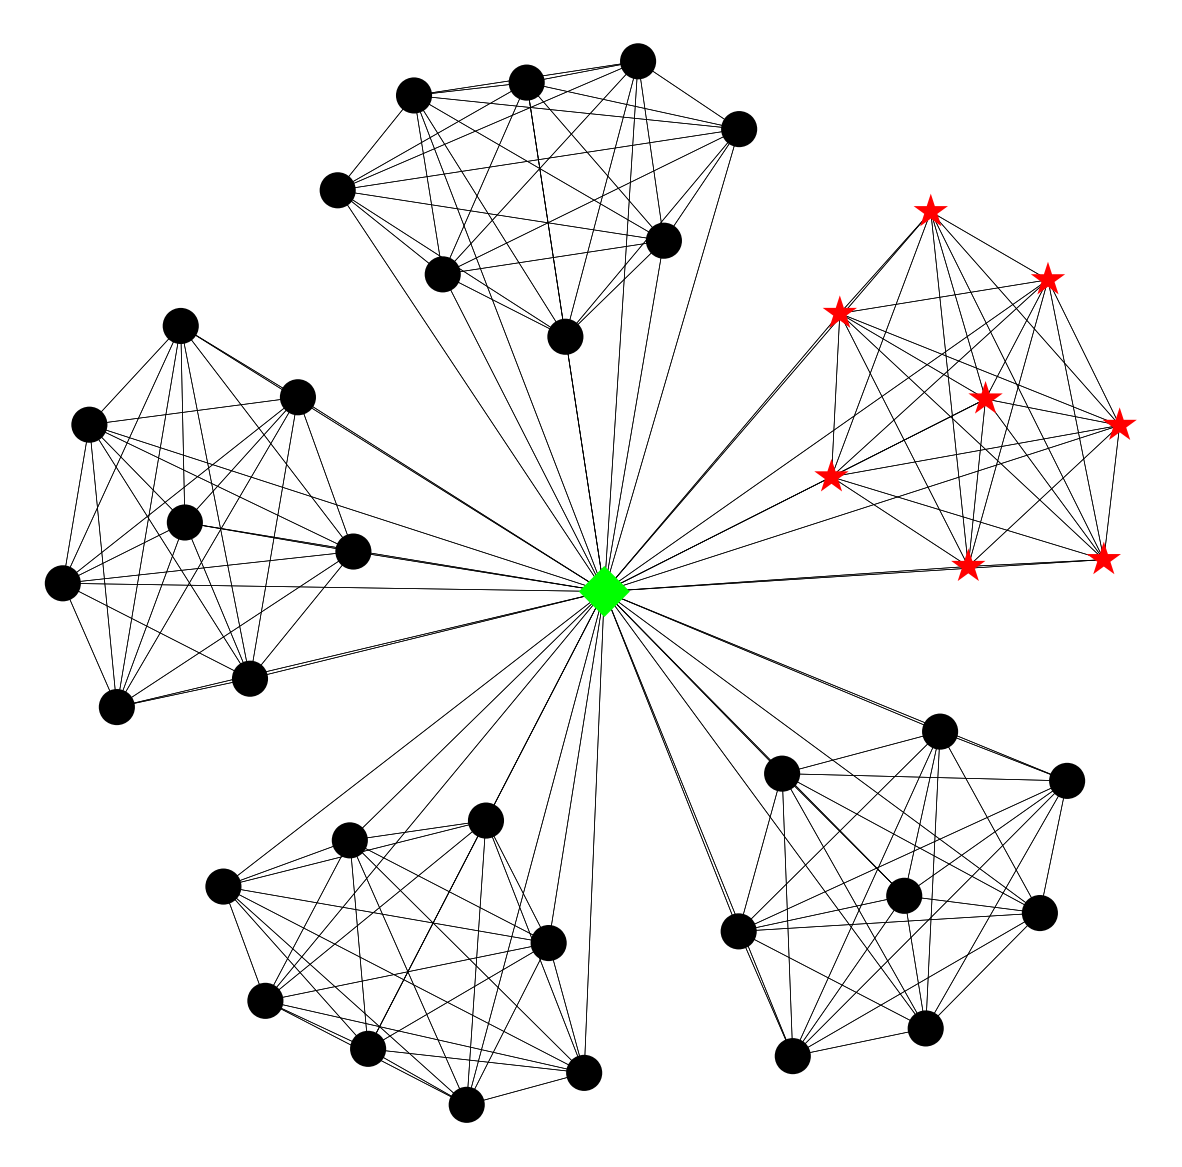
\includegraphics[width=0.3\linewidth]{media/From_ASONAM/Graphs/rep_soc_graph.png}\label{subfig:rep_soc_graph}}
    \hfill
    \subfloat[Ring of stars]{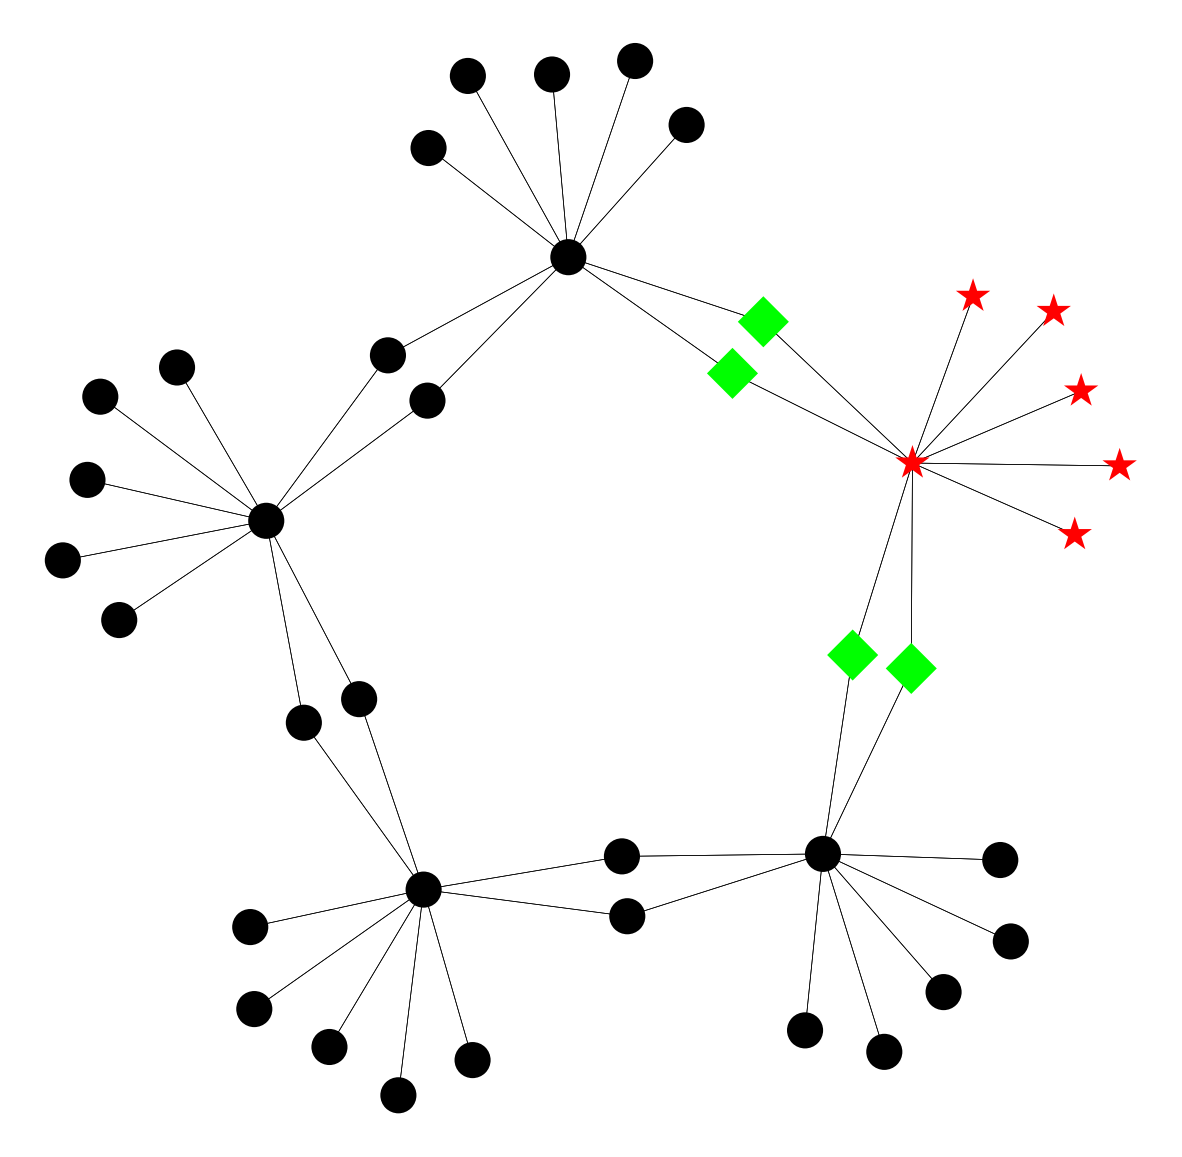
\includegraphics[width=0.3\linewidth]{media/From_ASONAM/Graphs/rep_ros_graph.png}\label{subfig:rep_ros_graph}}
    \hfill
    \subfloat[Toy Graph from SBM]{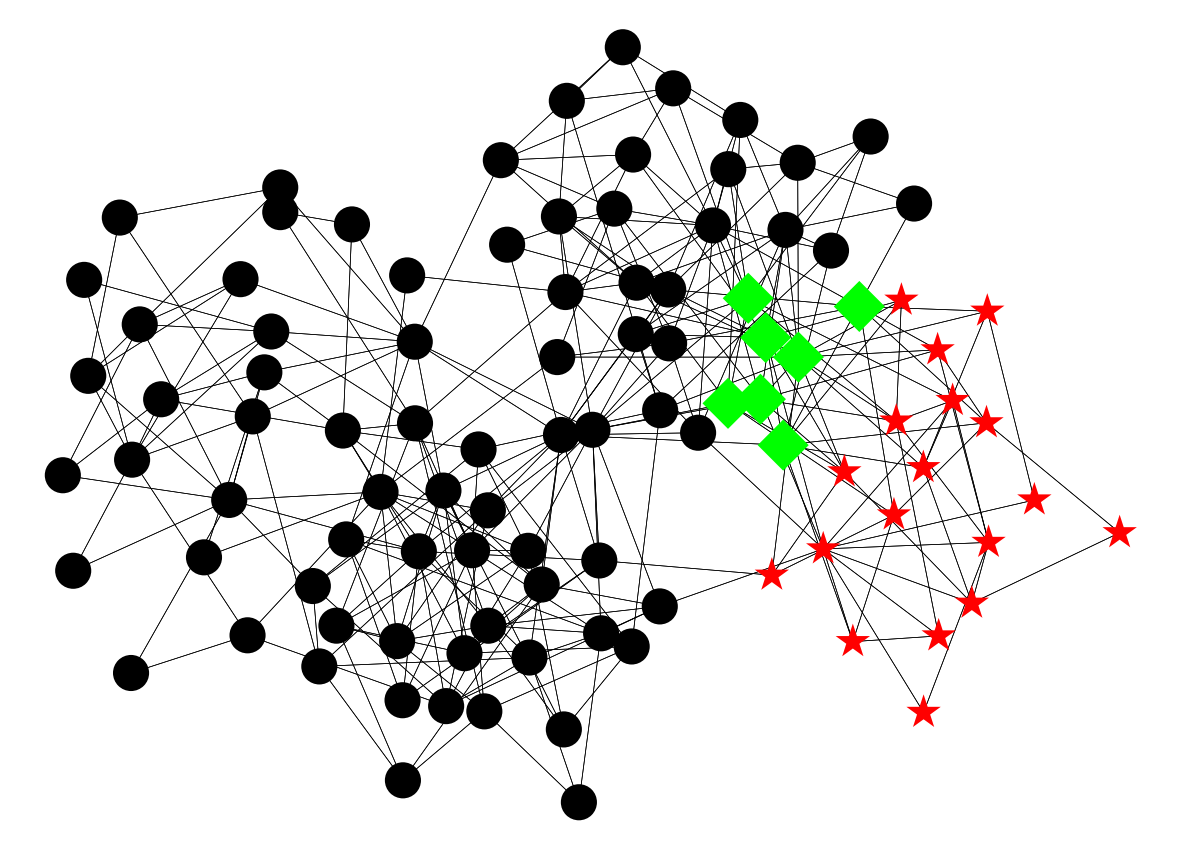
\includegraphics[width=0.3\linewidth]{media/From_ASONAM/Graphs/rep_toy_graph.png}\label{subfig:rep_toy_graph}}

    \subfloat[$\mat{\Pi} - \alpha \identity{n}$ matrix of the star of cliques]{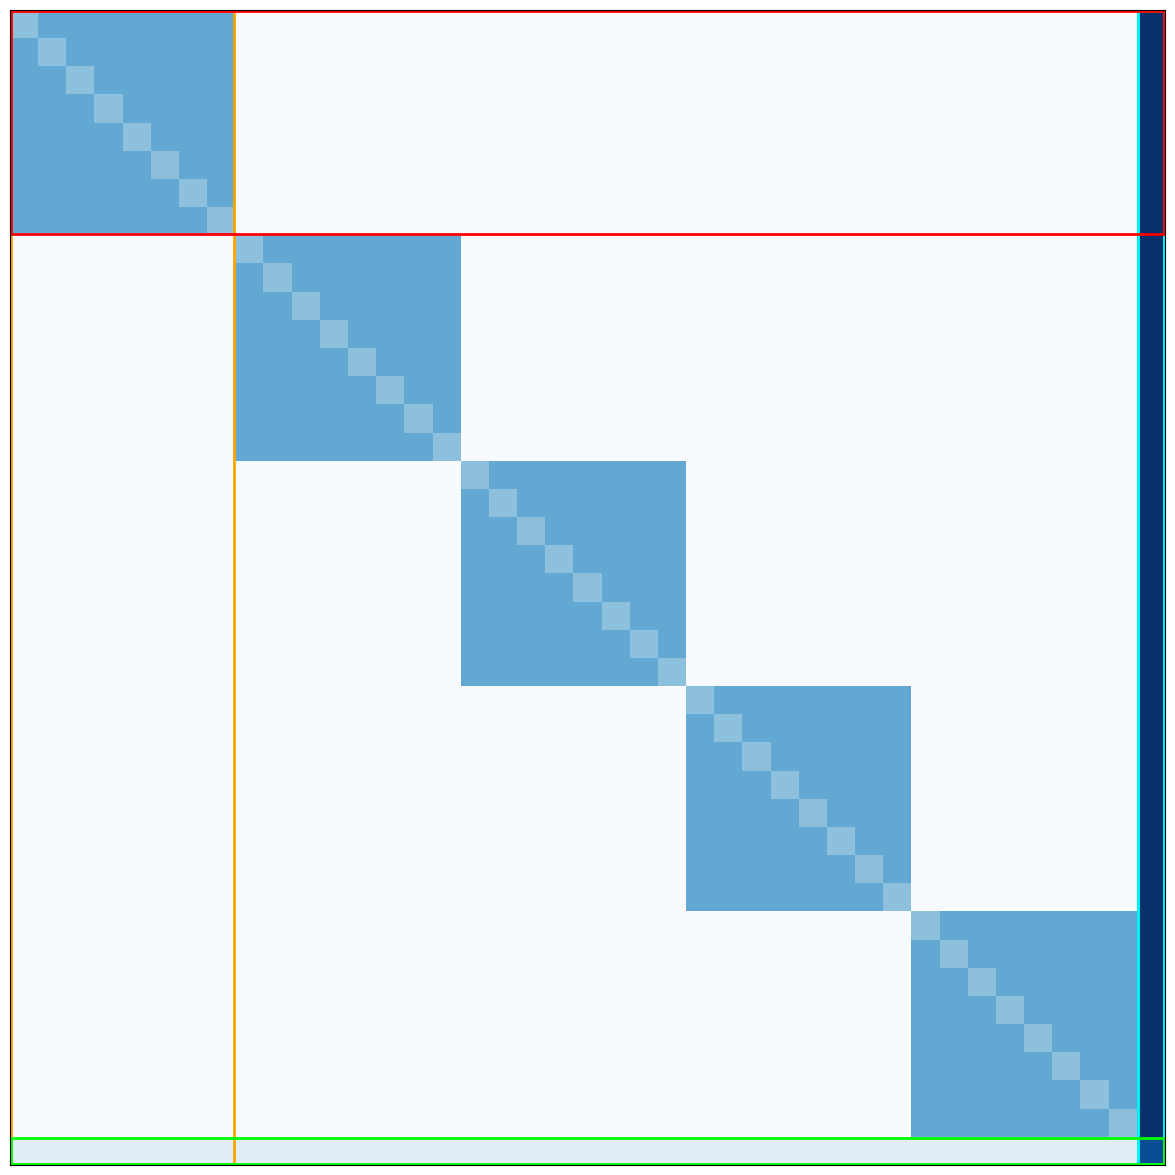
\includegraphics[width=0.3\linewidth]{media/From_ASONAM/PPR_matrices/ppr_mat_soc_graph.png}\label{subfig:ppr_mat_soc_graph}}
    \hfill
    \subfloat[$\mat{\Pi} - \alpha \identity{n}$ matrix of the ring of stars]{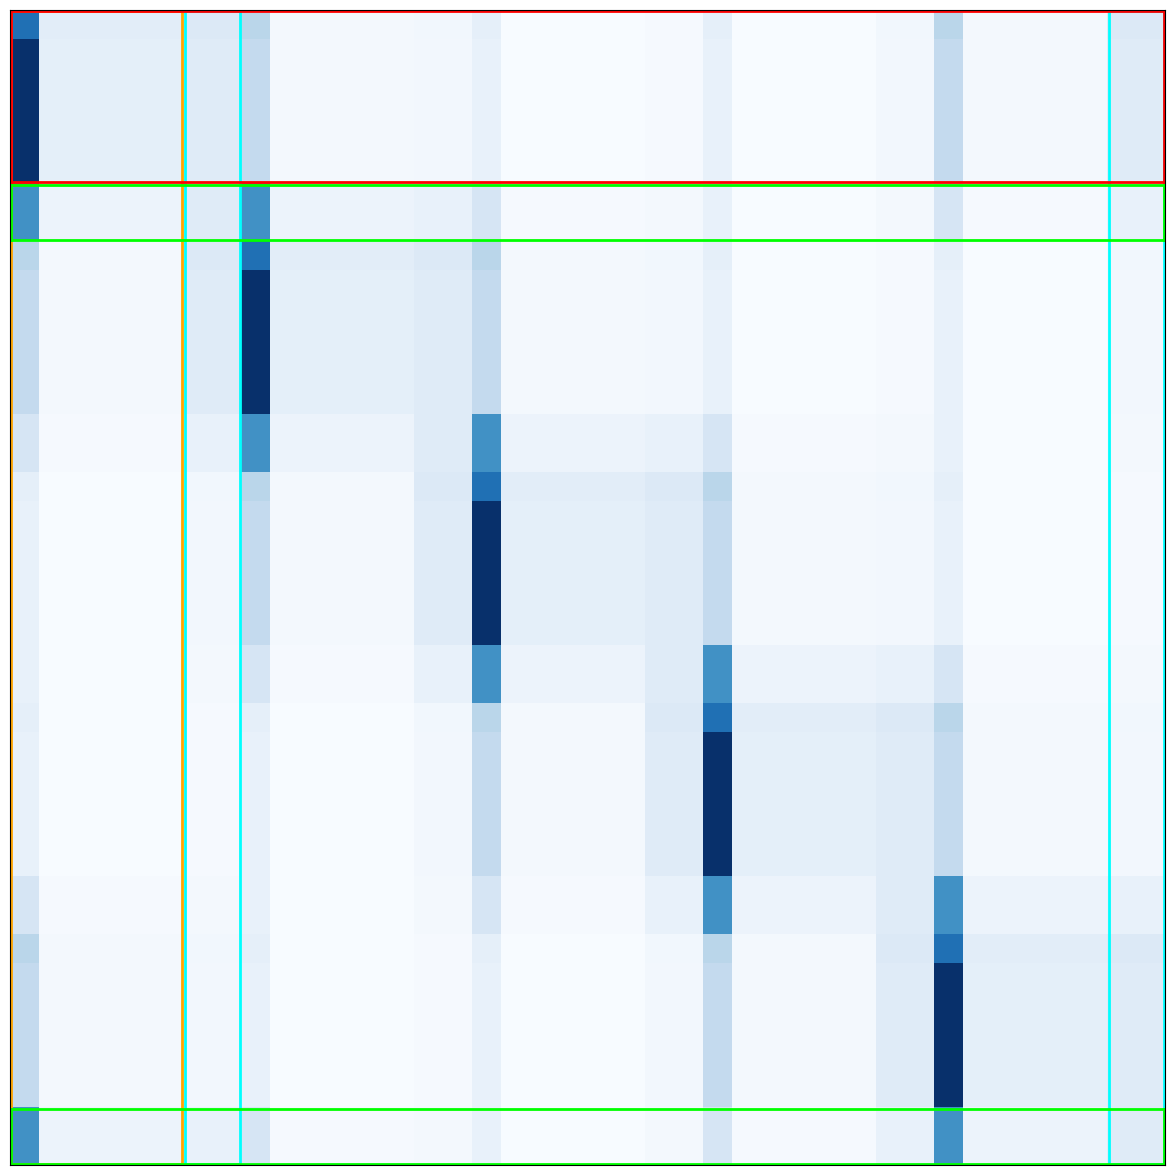
\includegraphics[width=0.3\linewidth]{media/From_ASONAM/PPR_matrices/ppr_mat_ros_graph.png}\label{subfig:ppr_mat_ros_graph}}
    \hfill
    \subfloat[$\mat{\Pi} - \alpha \identity{n}$ matrix of the toy graph from SBM]{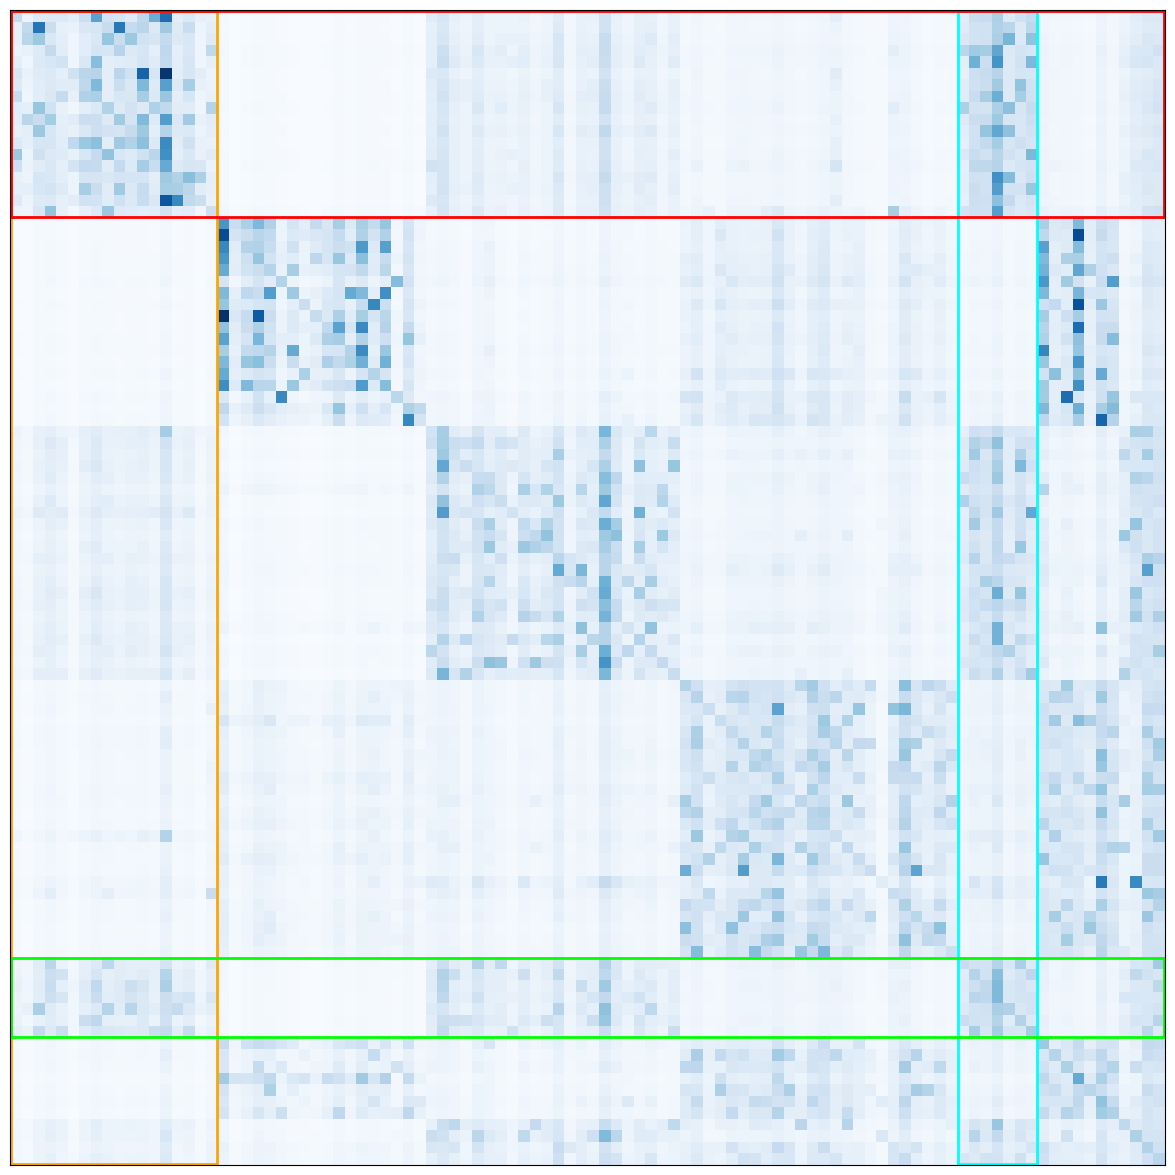
\includegraphics[width=0.3\linewidth]{media/From_ASONAM/PPR_matrices/ppr_mat_toy_graph.png}\label{subfig:ppr_mat_toy_graph}}
    %\subfloat[PPR matrix of the toy graph]{\includesvg[width=0.45\linewidth]{Figures/SBM_PPR.svg}\label{subfig:SBM_PPR}}
    \caption[Toy graphs and their respective $\mat{\Pi} - \alpha \identity{n}$ matrices]{Toy graphs and their respective $\mat{\Pi} - \alpha \identity{n}$ matrices. On each graph, a community is highlighted, the red stars vertices belonging exclusively to the community, and the green diamonds ones belonging both to the highlighted community and to at least one other. On each matrix, the rows and columns relative to the red star vertices are highlighted through red and orange boxes, and the rows and columns relative to the green diamond vertices are highlighted through green and cyan boxes.  We use $\mat{\Pi} - \alpha \identity{n}$ instead of $\mat{\Pi}$ for better readability.}
    \label{fig:graphs_PPR}
\end{figure*}

%One of the main advantages of the SVD, that make it especially attractive for embedding, is that it is known to filter out the noise in the data. More specifically, the SVD removes the small variations between data so that only the main patterns in the matrix are kept in the final result \cite{SVD_filtering_data}.
\todo{Use this paragraph in "our approach" part ?}

\subsection{Our approaches}\label{sec:approach}\todo{Approaches ? (plural ?)}
\subsubsection{Overview} \label{subsec:overview}
We introduce the new PAgeRank FActorization-based InTerpretable Embedding (\parfaite{}) method. It produces two embeddings, \newembLeft{} (left) and \newembRight{} (right).

Our method consists of three main parts. First, a truncated Singular Values Decomposition is performed on the centered PPR matrix. To overcome the issues of computing and representing the PPR matrix exactly for very large graphs, we employ a function $m$ that, given any vector $\vect{v}$, approximates the multiplication of the matrix with the vector. This results in two representations of the vertices as $\mat{U}\mat{\Sigma}$ and $\mat{V}\mat{\Sigma}$.

Then, vertices are clustered, with each vertex being represented by a concatenation of its left and right representation. This provides the central points of the communities in the space of these representations, stored in the matrix $\mat{C}$. Finally, our left and right embeddings, respectively \newembLeft{} and \newembRight{} are computed by projecting back these central points onto the original spaces. A pseudocode of our algorithm is shown in Algorithm~\ref{algo:emb}. 

\begin{algorithm}
    \caption{\parfaite{}}\label{algo:emb}
    \begin{algorithmic}[1]
    \Procedure{\parfaite{}}{$\mat{P}$: stochastic random walk matrix, $m_P$: function that approximate $\mat{\Bar{\Pi}}\vect{v}$ for any $\vect{v}$}
    %\KwResult{$\mat{C_l}, \mat{C_r}$ the left and right embeddings}
    \State $\mat{U}$, $\mat{\Sigma}$, $\mat{V}$ $\gets$ SVD($m_P$)
    \State clustering $\gets$ kmeans(concat( normalize($\mat{U}\mat{\Sigma}$), normalize($\mat{V}\mat{\Sigma}$)))
    \State $\mat{C} \gets$ clustering.clusters\_centers
    \State \newembLeft{} $ \gets \mat{U}\mat{C}_{\cdot, d:}^\top$
    \State\newembRight{} $ \gets \mat{V}\mat{C}_{\cdot, :d}^\top$
    \State \textbf{return} \newembLeft{}, \newembRight{}
    \EndProcedure
    \end{algorithmic}
\end{algorithm}

\subsubsection{Interpretation of the steps}\label{subsec:interpretation}


The \parfaite{} method relies on the well-established fact that the PPR vector of each vertex often contains large scores at dimensions corresponding to vertices it shares at least one community with, while it contains small scores at other dimensions \cite{Hollocou2017,Kloumann2014}. When we consider the PPR vector as a relevance scoring of the vertices of the graph wrt. the source vertex, it means that the vertices of the graph that are the most relevant to the source vertex are those which share a community with it.

This property strengthens the one stated by \cite{zhang_2020} that two nodes are likely to share a community not only if the PPR score from one node to the other is high, but especially if their PPR vectors are similar., meaning that they "agree with each other in terms of their personalized views about the network" \cite{zhang_2020}.


We illustrate this property with three toy graphs represented in Figure~\ref{fig:graphs_PPR}. The first two graphs provide ideal cases where we can find communities according to two natural community definitions: a) a clique, where each node is connected to every other node in the community,
and b) a star where all nodes but one are connected to a single node (e.g. they are connected to a same influencer in social media). In particular, Figure~\ref{subfig:rep_soc_graph} represents a star of cliques, while Figure~\ref{subfig:rep_ros_graph} represents a ring of stars. Observe that the communities in the graphs of Figure~\ref{fig:graphs_PPR} do \define{overlap}, which means that some nodes belong to several communities at the same time. On each graph represented in Figure~\ref{fig:graphs_PPR}, one community is outlined. Red star vertices are those that belong exclusively to the outlined community, while green diamond vertices belong to the outlined community and at least another one. The graph in Figure~\ref{subfig:rep_toy_graph} is built using the Stochastic Block Model (SBM) with 100 vertices, 300 edges, 4 communities, with each pair of vertices of a same community being $100$ times more likely to be connected than two vertices from different communities. As a result, in Figure~\ref{subfig:rep_toy_graph}, there are 19 vertices belonging to exactly two communities, 7 of which are depicted in green. 

Figures~\ref{subfig:ppr_mat_soc_graph}, \ref{subfig:ppr_mat_ros_graph} and~\ref{subfig:ppr_mat_toy_graph} show the corresponding PPR matrices. Recall that each row corresponds to some vertex $v$ and it represents the PPR vector of $v$, that is the PPR scores when $v$ is the source vertex of the random walk. Indeed, we can see that PPR vectors contain larger scores to vertices of a same community as the source node, generating "square" patterns in the matrices.

Similarly, we observe that the reversed PPR vectors (columns in the matrix) exhibit the same pattern of large scores inside the community and low scores outside.

However, there might be relatively few vertices that have very large PPR scores even if they do not share communities with other nodes. This is apparent in Figure~\ref{subfig:ppr_mat_ros_graph}, where we observe that the central nodes in the neighboring cliques have higher scores in the PPR vector of the studied community than other nodes in the same community. The reversed PPR is not affected by that issue.

To avoid this biais, we define the $\mat{\Bar{\Pi}}$ matrix obtained by centering the columns of $\mat{\Pi}$.\todo{Introduce the proba we are talking about}

\begin{property}
    \begin{equation*}
        \mat{\Bar{\Pi}}_{i, j} = \frac{1}{n}\proba{X_f = j}\big(\proba{X_0=i|X_f=j}-\proba{X_0 = i}\big)
    \end{equation*}
\end{property}

\begin{proof}
\begin{align*}
        \mat{\Bar{\Pi}}_{i, j} & =  \proba{X_f = j | X_0 = i} - \proba{X_f = j} \\
         & =  \frac{\proba{X_0 = i | X_f = j}\proba{X_f = j}}{
            \proba{X_0=i}
            %\underbrace{\proba{X_0=i}}_{1/n}
        }
         - \proba{X_f = j}
\end{align*}
\end{proof}

If we look at the rows of this new matrix, each entry is then the excess of probability to go to each vertex from the reference vertex, compared to the agnostic probability. If we look at the columns and because $\proba{X_f =j}$ is a constant along a column, each entry is proportional to the excess of probability to come from each vertex given that the walk arrived at the reference vertex.

Because the SVD only keeps the main patterns of the matrix it decomposes as we saw in section \todo{link section back svd}, we expect the result of the SVD to exhibit the typical rows and columns for each community, i.e. the patterns of the excess of probability to respectively come from and arrive into the community given that we respectively arrived into and came from the community.
We could then interpret these vectors as respectively the belonging of each node to the community and its relevance wrt. the community.

Our last problem is that, although the truncated SVD should make the community patterns in the matrix apparent, each dimension of the decomposition does usually not match a community, hindering the interpretation. To tackle this issue we perform a clustering on the vertices represented by the SVD, and we use the central points to obtain the desired representative vectors for each community. Note that, although the clustering itself is non-overlapping and non-fuzzy, the resulting vectors are fuzzy scoring of belonging and importance of the nodes in each community.\todo{Illustrate on toy graph?}

\subsubsection{Decomposition of the PPR matrix}
The PPR matrix is a dense matrix belonging to $\realset^{n\times n}$. In most cases of big graphs, this matrix is too big to be explicitly represented. As we saw in section \todo{Ref to back SVD}, most modern SVD algorithms don't require an explicit representation of the matrix $\mat{M}$ but only a function $m(\vect{v}) = \mat{M}\vect{v}$. We use a reduced form of equation \eqref{eq:ppr_mat_as_series} to approximate the PPR matrix.

\begin{equation}
    m(\vect{v}) = \mat{\Bar{\Pi}_l}\vect{v} = (\alpha \sum_{i=0}^l (1-\alpha)^i\mat{P}^i\vect{v}) - (\vect{\pi} \cdot \vect{v}) \vect{1}
\end{equation}
\noindent where $\vect{1}$ is the vector of which all entries equal $1$ and $\vect{\pi}$ is the (not-personalized) PageRank vector of the matrix.

We know from \cite{Kloumann2014} that a few steps are usually enough to compute an approximation of the PageRank vector that outlines the community of the node. We fix $l=10$ for the rest of this section.

\subsubsection{Finding the communities}
SVD provides representations that should, if used to reconstruct the matrix, contain only the main patterns of the matrix which are the communities. There is no reason however to think that the dimensions of the representations correspond themselves to communities. That is why we perform a clustering of the vertices using their SVD representations to find the communities. Since both matrices of the embedding provide relevant and distinct information, there is no reason to exclude one and therefore we use a concatenation of both sides as the vectors for the clustering. 
Unfortunately we did not have enough time during this thesis to study which clustering algorithm would perform best for this task, and we simply use the well-known k-means++ algorithm and its initialization variant k-means++.

As we saw before, the PPR and reversed PPR vectors for vertices of a same community are expected to have similar patterns of high and low entries, which correspond to similar directions of the vectors. They are however not supposed to have similar norms, especially for the reversed PPR for which the norm typically follows the importance of the vertex. To make the clustering algorithm work on directions and not on euclidean distance, both embeddings are normalized before concatenation and then the cosine similarity is used.

\subsubsection{Reconstructing the communities rows and columns}
The $\mat{U}\mat{\Sigma}$ and $\mat{V}\mat{\Sigma}$ embeddings are the projection of the columns and rows of the centered PPR matrix onto the singular spaces, e.g. for a vertex of the graph $w$, we have $ (\mat{U}\mat{\Sigma})_{w, \cdot} = \vect{\Bar{\pi}_w}^\top\mat{V}$. Therefore the clusters centers are the central columns and rows of each community, projected on the singular spaces. To reconstruct the true central columns and rows of the communities, which are the typical centered reversed PPR and centered PPR vectors for the community, we multiply by the transposed of the projection matrices, which are $\mat{U}$ and $\mat{V}$. Note that this reconstruction is not perfect because the dimensions of the singular spaces we use are smaller than the dimension of the original space.
\todo{Look at Galerkin method that can justify this way of doing}

\subsection{Experiments}\label{sec:exp}

Our main goal is to show that our method provides better interpretability scores than state-of-the-art approaches, while boasting similar results for a popular machine learning task in graph analysis, such as link prediction. 

\noindent\textbf{Datasets.}
We use two datasets that are available on the SNAP website \cite{SNAP_paper}. The first one named \textit{Wikispeedia} contains 4592 vertices, and 120~000 edges. 105 overlapping ground-truth community are given. The second one named \textit{Facebook} contains 10 graphs. We exclude 2 of them, numbered 698 and 3980, because they contain less than 128 nodes and we could therefore not compute the SVD for them using the same parameters used for the others. The remaining 8 graphs contain between 155 and 1035 vertices and between 3312 and 60050 edges. Between 7 and 46 overlapping ground-truth communities are given for each graph.

We also use our new WikipediaFr dataset that contains 2.52 millions vertices, 102 million edges and 2~700 ground-truth communities. To keep the dimension of the embeddings manageable however we only study the 117 communities that contain more than 10~000 vertices.

%We also release a new dataset with ground-truth communities\footnote{https://gitlab.telecom-paris.fr/gabriel.damay/WikipediaFRNetwork} (Wikipedia fr), constructed from all the pages of the French version of Wikipedia.\footnote{All the pages from the main space of Wikipedia, that is all the pages usually accessed by public, excluding discussions, user pages etc.} In such a graph, nodes represent Wikipedia pages while directed edges represent links between the corresponding Wikipedia pages. In the French version of Wikipedia, it is common to add links to so called ``portals'' at the end of the page which serve as reference pages for given topics and can be seen as ground-truth communities. %We observe that links to portals are more rare in the English version of Wikipedia, while portals are more semantically related to their corresponding Wikipedia pages than Wikipedia categories.
%Such novel graph contains 2.52 millions vertices, 102 million edges and 2~700 ground-truth communities. 
\todo{Make a section for WikipediaFr}

\noindent\textbf{Methods.} 
We evaluate our method against the two widely used algorithms for graph embedding HOPE and node2vec described in section \ref{subsec:embedding_history}.

We evaluate all methods in terms of the IS, BCI, CCI and CISIP metrics, discussed in section \ref{subsec:interpretability_explained}. However we consider the BCI and CCI results with a skepticism\todo{Check if results are good, and if they are say it.} because of the limitations due to their normalization, as explained in the aforementioned section.
We include in our experiments embeddings produced by the state-of-the-art node2vec and HOPE algorithms and our 2 new embeddings \newembLeft{} and \newembRight{}.

For node2vec, we use the most-used python3 implementation \cite{node2vec_impl}. We keep the default parameters, i.e. the number of walks is 200 per vertex, the length of the walks is 30 and the window size is 10.

For HOPE, we use the official implementation in Matlab\footnote{https://github.com/ZW-ZHANG/HOPE} provided by the authors of \cite{HOPE} that we reimplement in python3 (while using numpy and scipy), so as to provide a fair comparison with the other approaches. We keep all the constants and parameters as available in this implementation.
%\todo{Make the implementation available}

Our algorithm is implemented in python3 using mainly the numpy \cite{numpy} and scipy \cite{scipy} packages. The jump parameter $\alpha$ for the PPR algorithm is set to $\alpha=0.1$. The number $l$ of iterations to approximate the PPR matrix is set to $l=10$ and the dimension $D$ of the intermediate SVD is set to $D=128$.\todo{Rename dimension? $D$ is supposed to be the diagonal matrix}

For all embeddings %and in order to optimize the potential interpretability,
the dimension $K$ of the embedding is set to be the number $G$ of known ground-truth communities.

\noindent\textbf{Metrics.} We measure the interpretability of the methods using each of the metrics mentioned in the "metrics" part of the section \ref{subsec:interpretability_explained}. The Interpretability Scores (IS) are aggregated along the ground-truth groups using the max function, and then along the embedding dimensions using the sum function.
The size of the top and bottom sets considered for the Betweenness and Closeness Centrality Indices (BCI and CCI) are set to the size of the studied ground-truth group, as suggested by the original paper.
For CISIP, three smoothing functions $f$ are considered. The first one, that we call "identity" is the direct use of the binary belonging feature, the second one is the Mean Neighbors Belonging (MNB), that is the mean of the belonging features of the neighbors, and the last one is the PPR of the community.

The BCI and CCI are not computed for the WikipediaFr for performances reasons.

\subsection{Results}
The results are given in Table~\ref{tab:IS_scores} \todo{Add all results}and~\ref{tab:CISIP_scores}. Because of space limitation, only Facebook 107 and 1912, as parts with highest degree and order of Facebook, are presented, as well as Facebook 3437 because of the good performances of HOPE on this dataset with the CISIP-identity metric. The results for the other versions of Facebook are similar to what is presented.

As we see in these results, our algorithm's interpretability is much higher than node2vec's when evaluated using the Interpretability Score or any of the variants of CISIP. HOPE's interpretability is closer but still generally below \parfaite{}'s.

Our left embedding greatly outperforms the right one when using CISIP with the PPR smoothing, and this result was expected, as the left embedding is an approximation of the typical PPR vector of each clusters detected. The results are however equivalent between our two embeddings when compared using either the IS or CISIP with the identity smoothing, which both evaluate directly the matching between the embedding and the belonging features, or with the MNB smoothing. This is consistent with our interpretation that the left embedding represents which communities a vertex belongs to, while the right embedding measures somehow the ``importance'' of a vertex in a community.

\subsection{Is the clustering needed ?}
To check if the last step of our algorithm of clustering the data and computing the final embeddings is really needed, we compare our results to what we would have without the clustering step. To achieve this, we take the $\mat{U}\mat{\Sigma}$ and $\mat{V}\mat{\Sigma}$ results from the SVD, and we keep only the $G$ first dimensions to match the dimension of the \parfaite{} embeddings so that the dimension of this embedding is identical to the dimension of the \parfaite{} embeddings.

The results for IS and for CISIP with the three smoothing functions already used are presented in Table~\ref{tab:IS_SVD_scores} and~\ref{tab:CISIP_SVD_scores}. We see that in most cases the results of our \newembLeft{} and \newembRight{} outperform those before clustering, sometimes significantly (e.g. more than $0.1$ points of difference for the IS). This is especially true for the IS and CISIP with PPR smoothing. We note however that the SVD provides better results in several occurrences when compared to our embeddings using CISIP with the identity or the MNB smoothing.

Overall we conclude that \newembLeft{} and \newembRight{} do generally perform better than single SVD, i.e. without the clustering and reconstruction steps.

\subsection{Is our embedding efficient ?}
The method we propose mainly focuses on the interpretability of the embedding. This interpretability should however not come at the cost of an excessive loss of efficiency in the task the embedding helps solving.

We check the efficiency of \parfaite{} against HOPE and node2vec at the task of Link Prediction. We build test graphs by removing 0.1\% of the edges of a real-world graph. We store the pairs of vertices of these edges as "positive" pairs, and build a set of "negative" pairs by drawing the same number of pairs of vertices that are not connected by an edge.

The embedding of the test graph is computed and a score is attributed to each positive or negative pair of vertices using this embedding.

For HOPE, the score is the dot product of the left embedding of the first vertex in the pair and the right embedding of the second vertex. The score for \parfaite{} is similar but the left embedding of the first vertex is normalized to account for the entire use of the singular values on each side of the embedding. For node2vec, following \cite{groverNode2vecScalableFeature2016}, a Logistic Regression is trained on the test graph by representing the pairs with a concatenation of their vertice's embeddings.

We run this experiment on 10 test graph for both the Wikispeedia dataset and on the 1912 part of the Facebook dataset, as the part with the highest order. The mean results are given in Figure \ref{fig:lp_results}. As we can see, node2vec is outperformed by both HOPE and \parfaite{}. HOPE achieves similar results as \parfaite{} on Facebook~1912 and slightly better on Wikispeedia but overall we can say that the greater interpretability of \parfaite{} does not come at the cost of lower efficiency on the task of link prediction.

\begin{figure}
   \centering
    \subfloat[Wikispeedia]{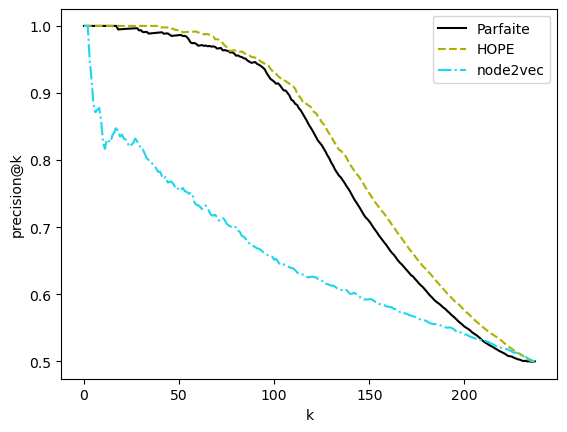
\includegraphics[width=0.5\linewidth]{media/From_ASONAM/LP/LP_results_wikispeedia.png}\label{subfig:lp_wikispeedia}}
    \subfloat[Facebook 1912]{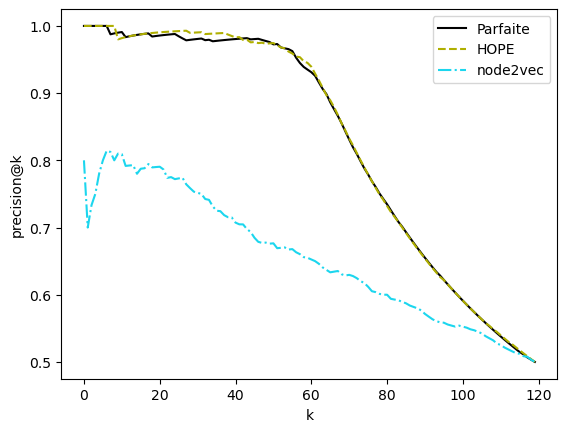
\includegraphics[width=0.5\linewidth]{media/From_ASONAM/LP/LP_results_facebook.png}\label{subfig:lp_facebook}}
    \caption[Precision@k results of the Link Prediction experiment]{Mean Precision@k of the Link Prediction on 20 test graphs built from the Wikispeedia and Facebook 1912 datasets}
    \label{fig:lp_results}
\end{figure}

\section{Conclusion and future work}\label{sec:conclusion}
We have presented \parfaite{}, a novel graph embedding algorithm and we have evaluated its interpretability against the state-of-the-art node2vec and HOPE algorithms. We also presented the new interpretability score CISIP to assure that interpretations are well-separated and non-redundant.
Our approach relies on the clustering of the vertex embeddings for which we use the $k$-means algorithm. An interesting direction for future work would be to study whether other clustering methods provide better results. We have also seen that, although the clustering phase increases the interpretability of our embedding, in some rare cases clustering might have a negative impact on the interpretability. It would be interesting to have a better understanding of this phenomenon which could pave the way for a more effective approach.  Finally, the CISIP metric contains a smoothing function as a parameter and it would be interesting to study the properties of various functions for this task and what they imply in terms of interpretability of the embedding at hand.

\begin{table}[t]
    \caption{Interpretability Score results for \parfaite{}, HOPE and node2vec}
    \begin{center}
        \begin{tabular}{l|c|c|c|c|c}
            \hline
            \textbf{Dataset} & \multicolumn{2}{|c|}{\textbf{\parfaite{}}} & \multicolumn{2}{|c|}{\textbf{HOPE}} & \textbf{node2vec}\\
            & left & right & left & right\\
            \hline
Wikispeedia  &  \textbf{0.389} & 0.375 & 0.200 & 0.266 & 0.139\\
%\hline
Facebook 0 & 0.520 & \textbf{0.567} & 0.529 & 0.530 & 0.429\\
%\hline
Facebook 107 & \textbf{0.626} & 0.601 & 0.550 & 0.550 & 0.323\\
%\hline
Facebook 348 & \textbf{0.968} & 0.928 & 0.888 & 0.888 & 0.895\\
%\hline
Facebook 414 & 0.854 & \textbf{0.861} & 0.683 & 0.683 & 0.414\\
%\hline
Facebook 686 & \textbf{0.736} & 0.730 & 0.650 & 0.650 & 0.617\\
%\hline
Facebook 1684 & \textbf{0.863} & 0.807 & 0.572 & 0.572 & 0.304\\
%\hline
Facebook 1912 & \textbf{0.766} & 0.764 & 0.603 & 0.603 & 0.348\\
%\hline
Facebook 3437 & 0.430 & \textbf{0.759} & 0.429 & 0.429 & 0.188\\
%\hline
WikipediaFr  &  0.040 & \textbf{0.083} & 0.041 & \textbf{0.083} & *\\
\hline
        \end{tabular}
    \end{center}
    \label{tab:IS_scores}
    * The embedding for this graph with node2vec as been stopped after 36h of computation.
\end{table}



\begin{table}[t]
\caption{CISIP results for \parfaite{}, HOPE and node2vec}
\begin{center}
\begin{tabular}{l|c|c|c|c|c}
\hline
%\textbf{Dataset} & \textbf{\newembLeft{}} & \textbf{\newembRight{}} & \textbf{node2vec} & \textbf{HOPE (l)} & \textbf{HOPE (r)}\\
\textbf{Dataset} & \multicolumn{2}{|c|}{\textbf{\parfaite{}}} & \multicolumn{2}{|c|}{\textbf{HOPE}} & \textbf{node2vec}\\
& left & right & left & right\\
\hline
\multicolumn{6}{c}{No smoothing (identity function)}\\
\hline
Wikispeedia  &  \textbf{0.429} & 0.414 & 0.339 & 0.318 & 0.255 \\
%\hline
Facebook 0 & \textbf{0.333} & 0.311 & 0.233 & 0.232 & 0.248 \\
%\hline
Facebook 107 & 0.403 & \textbf{0.408} & 0.316 & 0.316 & 0.234 \\
%\hline
Facebook 348 & 0.561 & \textbf{0.566} & 0.524 & 0.524 & 0.252\\
%\hline
Facebook 414 & 0.545 & \textbf{0.605} & 0.540 & 0.540 & 0.283\\
%\hline
Facebook 686 & \textbf{0.527} & 0.489 & 0.384 & 0.384 & 0.295\\
%\hline
Facebook 1684 & 0.483 & \textbf{0.493} & 0.369 & 0.369 & 0.264  \\
%\hline
Facebook 1912 & 0.401 & \textbf{0.425} & 0.352 & 0.353 & 0.266\\
%\hline
Facebook 3437 & 0.300 & 0.310 & \textbf{0.331} & \textbf{0.331} & 0.256\\
%\hline
WikipediaFr  &  0.350 & \textbf{0.376} & 0.339 & 0.353 & *\\
\hline
\multicolumn{6}{c}{Smoothing with MNB}\\
\hline
Wikispeedia  &  0.431 & \textbf{0.508} & 0.282 & 0.369 & 0.105 \\
%\hline
Facebook 0 & \textbf{0.436} & 0.434 & 0.230 & 0.230 & 0.028 \\
%\hline
Facebook 107 & \textbf{0.545} & 0.515 & 0.384 & 0.384 & 0.161\\
%\hline
Facebook 348 & \textbf{0.582} & 0.509 & 0.349 & 0.349 & 0.105\\
%\hline
Facebook 414 & \textbf{0.627} & 0.584 & 0.474 & 0.474 & 0.084\\
%\hline
Facebook 686 & \textbf{0.475} & 0.400 & 0.234 & 0.234 & 0.102\\
%\hline
Facebook 1684 & \textbf{0.539} & 0.532 & 0.389 & 0.389 & 0.122\\
%\hline
Facebook 1912 & 0.504 & \textbf{0.511} & 0.269 & 0.267 & 0.029\\
%\hline
Facebook 3437 & 0.513 & \textbf{0.524} & 0.373 & 0.373 & 0.067\\
%\hline
WikipediaFr  &  0.272 & \textbf{0.499} & 0.400 & 0.493 & *\\
\hline
\multicolumn{6}{c}{Smoothing with PPR}\\
\hline
Wikispeedia  &  0.449 & \textbf{0.516} & 0.189 & 0.174 & 0.012\\
%\hline
Facebook 0 & \textbf{0.429} & \textbf{0.429} & 0.143 & 0.138 & 0.074 \\
%\hline
Facebook 107 & \textbf{0.585} & 0.576 & 0.304 & 0.304 & 0.093 \\
%\hline
Facebook 348 & 0.633 & \textbf{0.682} & 0.510 & 0.510 & 0.071\\
%\hline
Facebook 414 & 0.589 & \textbf{0.774} & 0.531 & 0.531 & 0.283\\
%\hline
Facebook 686 & 0.454 & \textbf{0.550} & 0.285 & 0.285 & 0.106\\
%\hline
Facebook 1684 & 0.538 & \textbf{0.649} & 0.393 & 0.393 & 0.085 \\
%\hline
Facebook 1912 & 0.557 & \textbf{0.633} & 0.278 & 0.279 & 0.101\\
%\hline
Facebook 3437 & 0.568 & \textbf{0.688} & 0.402 & 0.402 & 0.073\\
%\hline
WikipediaFr  &  \textbf{0.123} & -0.067 & 0.049 & -0.015 & *\\
\hline
        \end{tabular}
    \end{center}
    \label{tab:CISIP_scores}
\end{table}

\begin{table}[t]
    \caption[Interpretability Score results for the SVD of the PPR matrix]{Interpretability Score results for the SVD of the PPR matrix. The results in bold as those at least as good as the related \parfaite{} results}
    \begin{center}
        \begin{tabular}{l|c|c}
            \hline
            \textbf{Dataset} & \textbf{SVD (left)} & \textbf{SVD (right)}\\
            \hline
Wikispeedia  & 0.234 & 0.204\\
%\hline
Facebook 0 & \textbf{0.538} & \textbf{0.593}\\
%\hline
Facebook 107 & 0.538 & 0.516\\
%\hline
Facebook 348 & 0.923 & \textbf{0.928}\\
%\hline
Facebook 414 & 0.808 & 0.812\\
%\hline
Facebook 686 & 0.690 & 0.696\\
%\hline
Facebook 1684 & 0.792 & 0.768\\
%\hline
Facebook 1912 & 0.589 & 0.604\\
%\hline
Facebook 3437 & 0.270 & 0.463\\
%\hline
WikipediaFr  & \textbf{0.043} & 0.061\\
\hline
        \end{tabular}
    \end{center}
    \label{tab:IS_SVD_scores}
\end{table}

\begin{table}[t]
\caption[CISIP results for the SVD of the PPR matrix]{CISIP results for the SVD of the PPR matrix. The results in bold as those at least as good as the related \parfaite{} results}
\begin{center}
\begin{tabular}{l|c|c}
\hline
\textbf{Dataset} & \textbf{SVD (left)} & \textbf{SVD (right)}\\
\hline
\multicolumn{3}{c}{No smoothing (identity function)}\\
\hline
Wikispeedia  & 0.363 & 0.362\\
%\hline
Facebook 0 & 0.333 & \textbf{0.360}\\
%\hline
Facebook 107 & \textbf{0.493} & \textbf{0.464}\\
%\hline
Facebook 348 & 0.520 & 0.525\\
%\hline
Facebook 414 & \textbf{0.545} & 0.549\\
%\hline
Facebook 686 & 0.438 & 0.440\\
%\hline
Facebook 1684 & \textbf{0.532} & \textbf{0.545}\\
%\hline
Facebook 1912 & 0.377 & 0.392\\
%\hline
Facebook 3437 & \textbf{0.304} & \textbf{0.337}\\
%\hline
WikipediaFr  & \textbf{0.350} & \textbf{0.381}\\
\hline
\multicolumn{3}{c}{Smoothing with MNB}\\
\hline
Wikispeedia  & 0.280 & 0.369\\
%\hline
Facebook 0 & 0.330 & 0.395\\
%\hline
Facebook 107 & \textbf{0.596} & \textbf{0.571}\\
%\hline
Facebook 348 & 0.404 & 0.412\\
%\hline
Facebook 414 & 0.431 & 0.404\\
%\hline
Facebook 686 & 0.320 & 0.337\\
%\hline
Facebook 1684 & 0.512 & 0.493\\
%\hline
Facebook 1912 & 0.299 & 0.320\\
%\hline
Facebook 3437 & 0.429 & 0.443\\
%\hline
WikipediaFr  & 0.259 & \textbf{0.502}\\
\hline
\multicolumn{3}{c}{Smoothing with PPR}\\
\hline
Wikispeedia  & 0.244 & 0.202\\
%\hline
Facebook 0 & 0.284 & 0.356\\
%\hline
Facebook 107 & \textbf{0.609} & \textbf{0.604}\\
%\hline
Facebook 348 & 0.449 & 0.485\\
%\hline
Facebook 414 & 0.527 & 0.541\\
%\hline
Facebook 686 & 0.378 & 0.407\\
%\hline
Facebook 1684 & 0.511 & 0.549\\
%\hline
Facebook 1912 & 0.319 & 0.320\\
%\hline
Facebook 3437 & 0.419 & 0.421\\
%\hline
WikipediaFr  & \textbf{0.150} & \textbf{-0.011}\\
\hline
\end{tabular}
\end{center}
\label{tab:CISIP_SVD_scores}
\end{table}

\section{A practical application: Detecting communities on a Youtube graph}
We teamed up with a company specialized in Youtube economics and data to extract a bipartite graph of Youtube. A \define{bipartite graph} is a graph in which the nodes are split into two parts and a node from one part can only share an edge with nodes of the other part. Each part usually represent a type of real-word entity. For example here one part represents the Youtube users while the other part represented Youtube videos. An edge represented the fact that the user had commented the video and it was weighted by the number of comments. However, due to technical limitations, we only had the last 15~000 comments on the videos of a same Youtube channel at the time of the scrapping.

The goal was to separate the graph into \define{clusters}, i.e. groups of nodes densely connected to one another, and sparsely connected to the rest of the graph. The graph had many small connected components and also some series of users connected to only a few videos, themselves connected to a few users. To remove these less interesting parts that made the clustering more difficult, we kept only the \define{$k$-core} of the graph, i.e. the maximal subgraph in which every node have at least $k$ neighbors. The values of $k$ we have considered $2$, $5$ and $10$. 

Then we tried two clustering methods in the graph. The first one computed a spectral embedding and then performed a k-means clustering on the resulting embedding. The second one used the Louvain algorithm, which is a well-known graph clustering algorithm, to cluster the data.

We presented the results as a small and easy website to help reading and browsing them\todo{Add screenshot}.

Unfortunately, the manual analysis of the results revealed poor performances. We worked with researchers interested in sociology who had partially clustered the videos and who did not find a convincing matching between their work and the results. After analysing the data, we think that the limitation to the last 15~000 comments on the videos of a same Youtube channel removed a lot of information. For example we probably lost a lot of times when a same user who was very loyal to a channel had commented on most of the videos at the time of their publication, because those comments would have been old and therefore "erased" by new comments.
